%=======================================================
%	PACKAGES AND THEMES
%=======================================================
\documentclass[8pt]{beamer}
\mode<presentation> {
\usepackage{etex}
\usetheme{Boadilla}
\definecolor{navyblue}{rgb}{0.0, 0.0, 0.5}
\definecolor{dkgreen}{rgb}{0,0.6,0}
\definecolor{gray}{RGB}{64, 64, 64}
\definecolor{teal}{RGB}{0, 102, 102}
\definecolor{mauve}{rgb}{0.58,0,0.82}
\usecolortheme[named = navyblue]{structure}
\setbeamercolor{normal text}{fg = gray}
\setbeamercolor{frametitle}{fg = white, bg = navyblue}
\setbeamerfont{framesubtitle}{size = \normalsize}
\setbeamerfont{caption}{size=\footnotesize}
\setbeamercolor{page number in head/foot}{fg = gray}
\setbeamertemplate{footline}%[frame number]
}


\usepackage{graphicx} % Allows including images
\usepackage{booktabs} % Allows the use of \toprule, \midrule and \bottomrule in tables
\usepackage{multicol}
\usepackage[export]{adjustbox}
\usepackage{colortbl}
\usepackage{graphicx} 

\usepackage{tikz}
\usepackage{fancybox}
\usepackage[absolute, overlay]{textpos}
\usepackage{multirow}
\usepackage{siunitx}
\usepackage{tcolorbox}


\usepackage{tikz}
\usepackage{calc}
\newlength{\outerradius}
\newlength{\innerradius}
\setlength{\outerradius}{0.50cm}
\setlength{\innerradius}{0.35cm}

%Damit wir Quellcode nutzen können.
\usepackage{listings}
\lstset{numbers=left,
	numberstyle=\tiny,
	numbersep=5pt,
	breaklines=true,
	showstringspaces=false,
	frame=l ,
	xleftmargin=15pt,
	xrightmargin=15pt,
	basicstyle=\ttfamily\scriptsize,
	stepnumber=1,
	keywordstyle=\color{blue},          % keyword style
  	commentstyle=\color{dkgreen},       % comment style
  	stringstyle=\color{mauve}         % string literal style
}
%Sprache Festelegen
\lstset{language=R}


%=======================================================
%	TITLE PAGE
%=======================================================

\title{\textbf{Innovation Networks}\\
	      {\color{teal}{--Seminar--}}}

\author{Yasemin Aslan}

\institute
{
SPRU (Science Policy Research Unit) \\
Business School\\
University of Sussex \\

\medskip

\medskip

\medskip

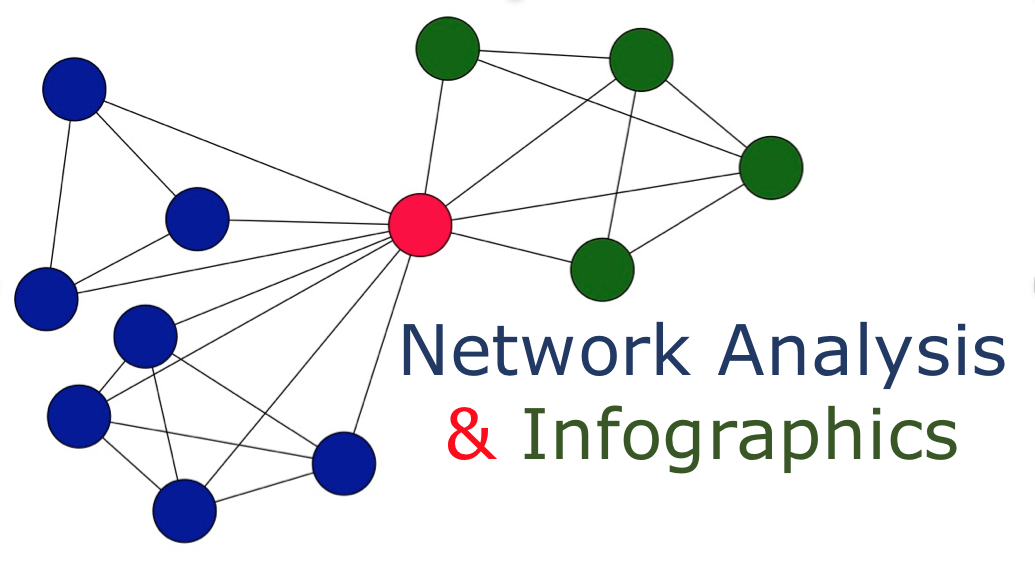
\includegraphics[width=2.5cm]{../_shared_pics/logo}

\medskip

\textit{{\color{dkgreen}{Week 9: 25 March 2022}}}\\
}


\date{} % Date, can be changed to a custom date

\begin{document}

\begin{frame}
\titlepage % Print the title page as the first slide

\begin{textblock*}{10pt}(0pt, 0.9\textheight)

\includegraphics[width=4cm]{../_shared_pics/SPRU.png}
\end{textblock*}

\end{frame}






%=======================================================
%	Learning outcomes
%=======================================================


\begin{frame}
\frametitle{\insertsection}
\framesubtitle{Learning Outcomes}

\centering
\begin{tabular}{lp{5.5cm}l}
\toprule
\multicolumn{2}{l}{\textbf{Learning outcome}} & \textbf{Assessment mode}\\
\hline
\\
1 & 
Explain the concept of network and list the main network indicators & 
ESS\\
\\
\rowcolor{green!20}2 &  
Describe and apply the major techniques for the collection of network data and their statistical analysis & 
ESS, GPN + GWS\\
\\
\rowcolor{green!20}3 & 
Identify the main characteristics of networks by means of network measures  & 
ESS, GPN + GWS\\
\\
4 &
Employ network analysis techniques to produce network data-based infographics & 
GPN + GWS\\
\\
\bottomrule
\multicolumn{3}{l}{\scriptsize Note: ESS: Essay; GPN: Group Presentation; GWS: Group Written Submission}\\
\end{tabular}

\end{frame}

%------------------------------------------------


%=======================================================
%	Intro slides
%=======================================================
\section*{Overview}
%------------------------------------------------

\begin{frame}
\frametitle{\insertsection}
\tableofcontents[hideallsubsections]
\end{frame}

%------------------------------------------------




%=======================================================
% Innovation network [recap]
%=======================================================
\section{Innovation network [recap]}
%------------------------------------------------

\bgroup
\setbeamercolor{background canvas}{bg = navyblue}
\begin{frame}[plain]{}
\begin{center}
\color{white}{\Huge\insertsection}
\end{center}
\end{frame}
\egroup

%------------------------------------------------

\begin{frame}
\frametitle{\insertsection}
\framesubtitle{Mapping}


Network analysis has been extensively used in {\color{blue}{bibliometrics/scientometrics}} to map science and technology
		
\medskip

\begin{itemize}
\item  {\color{blue}{Mapping of collaboration}}
		\begin{itemize}
		\item Co-authorship data (publications)
		\item Co-invention data (patents)
		\end{itemize}
		
\medskip

\item  {\color{blue}{Mapping of cognitive connections}}
 	    \begin{itemize}
		\item Citation analysis
    			\begin{itemize}
    			\item Direct citation analysis 
    			\item Co-citation analysis 
    			\item Bibliographic coupling 
    			\end{itemize}
		\item Co-word analysis
		\item Overlay mapping 
		\end{itemize}
		
\end{itemize}

\end{frame}

%------------------------------------------------




%=======================================================
% Introduction to VOSviewer
%=======================================================
\section{Introduction to VOSviewer}
%------------------------------------------------

\bgroup
\setbeamercolor{background canvas}{bg = navyblue}
\begin{frame}[plain]{}
\begin{center}
\color{white}{\Huge\insertsection}
\end{center}
\end{frame}
\egroup

%------------------------------------------------

\begin{frame}
\frametitle{\insertsection}

\begin{center}

\includegraphics[height=1.5cm]{vos_logo}\\
\url{http://www.VOSviewer.com/}
\end{center}

\begin{itemize}
\item Developed by van Eck and Waltman (CWTS, University of Leiden) 
\item Runs on {\color{blue}{Windows}}, {\color{blue}{Linux}}, {\color{blue}{Mac OSX}}
\item Relatively {\color{blue}{user-friendly}}
\item Can analyse {\color{blue}{scientometric data}}
\item Can import {\color{blue}{raw data}} from Web of Science, Scopus, PubMed
\item Capable of analysing {\color{blue}{relatively large networks}}
\item Operation cannot be easily {\color{red}{automated}}

\end{itemize}

\end{frame}

%------------------------------------------------

\begin{frame}
\frametitle{\insertsection}
\framesubtitle{Interfaces}

\begin{itemize}

\item {\color{blue}{Top}} tab 
    \begin{itemize}
    \item Network visualisation
    \item Overlay visualisation
    \item Density visualisation
    \end{itemize}

 \medskip

\item {\color{blue}{Left-hand side}} tab 
    \begin{itemize}
    \item load/sace data and maps
    \item analyse data
    \item explore clusters
    \end{itemize}

\medskip

\item {\color{blue}{Right-hand side}} tab
    \begin{itemize}
    \item Visualisation
    \item Labels
    \item Lines
    \item Colors
    \end{itemize}

\end{itemize}

\end{frame}

%------------------------------------------------

\begin{frame}
\frametitle{\insertsection}


\includegraphics[height=0.5cm]{vos_logo}\\
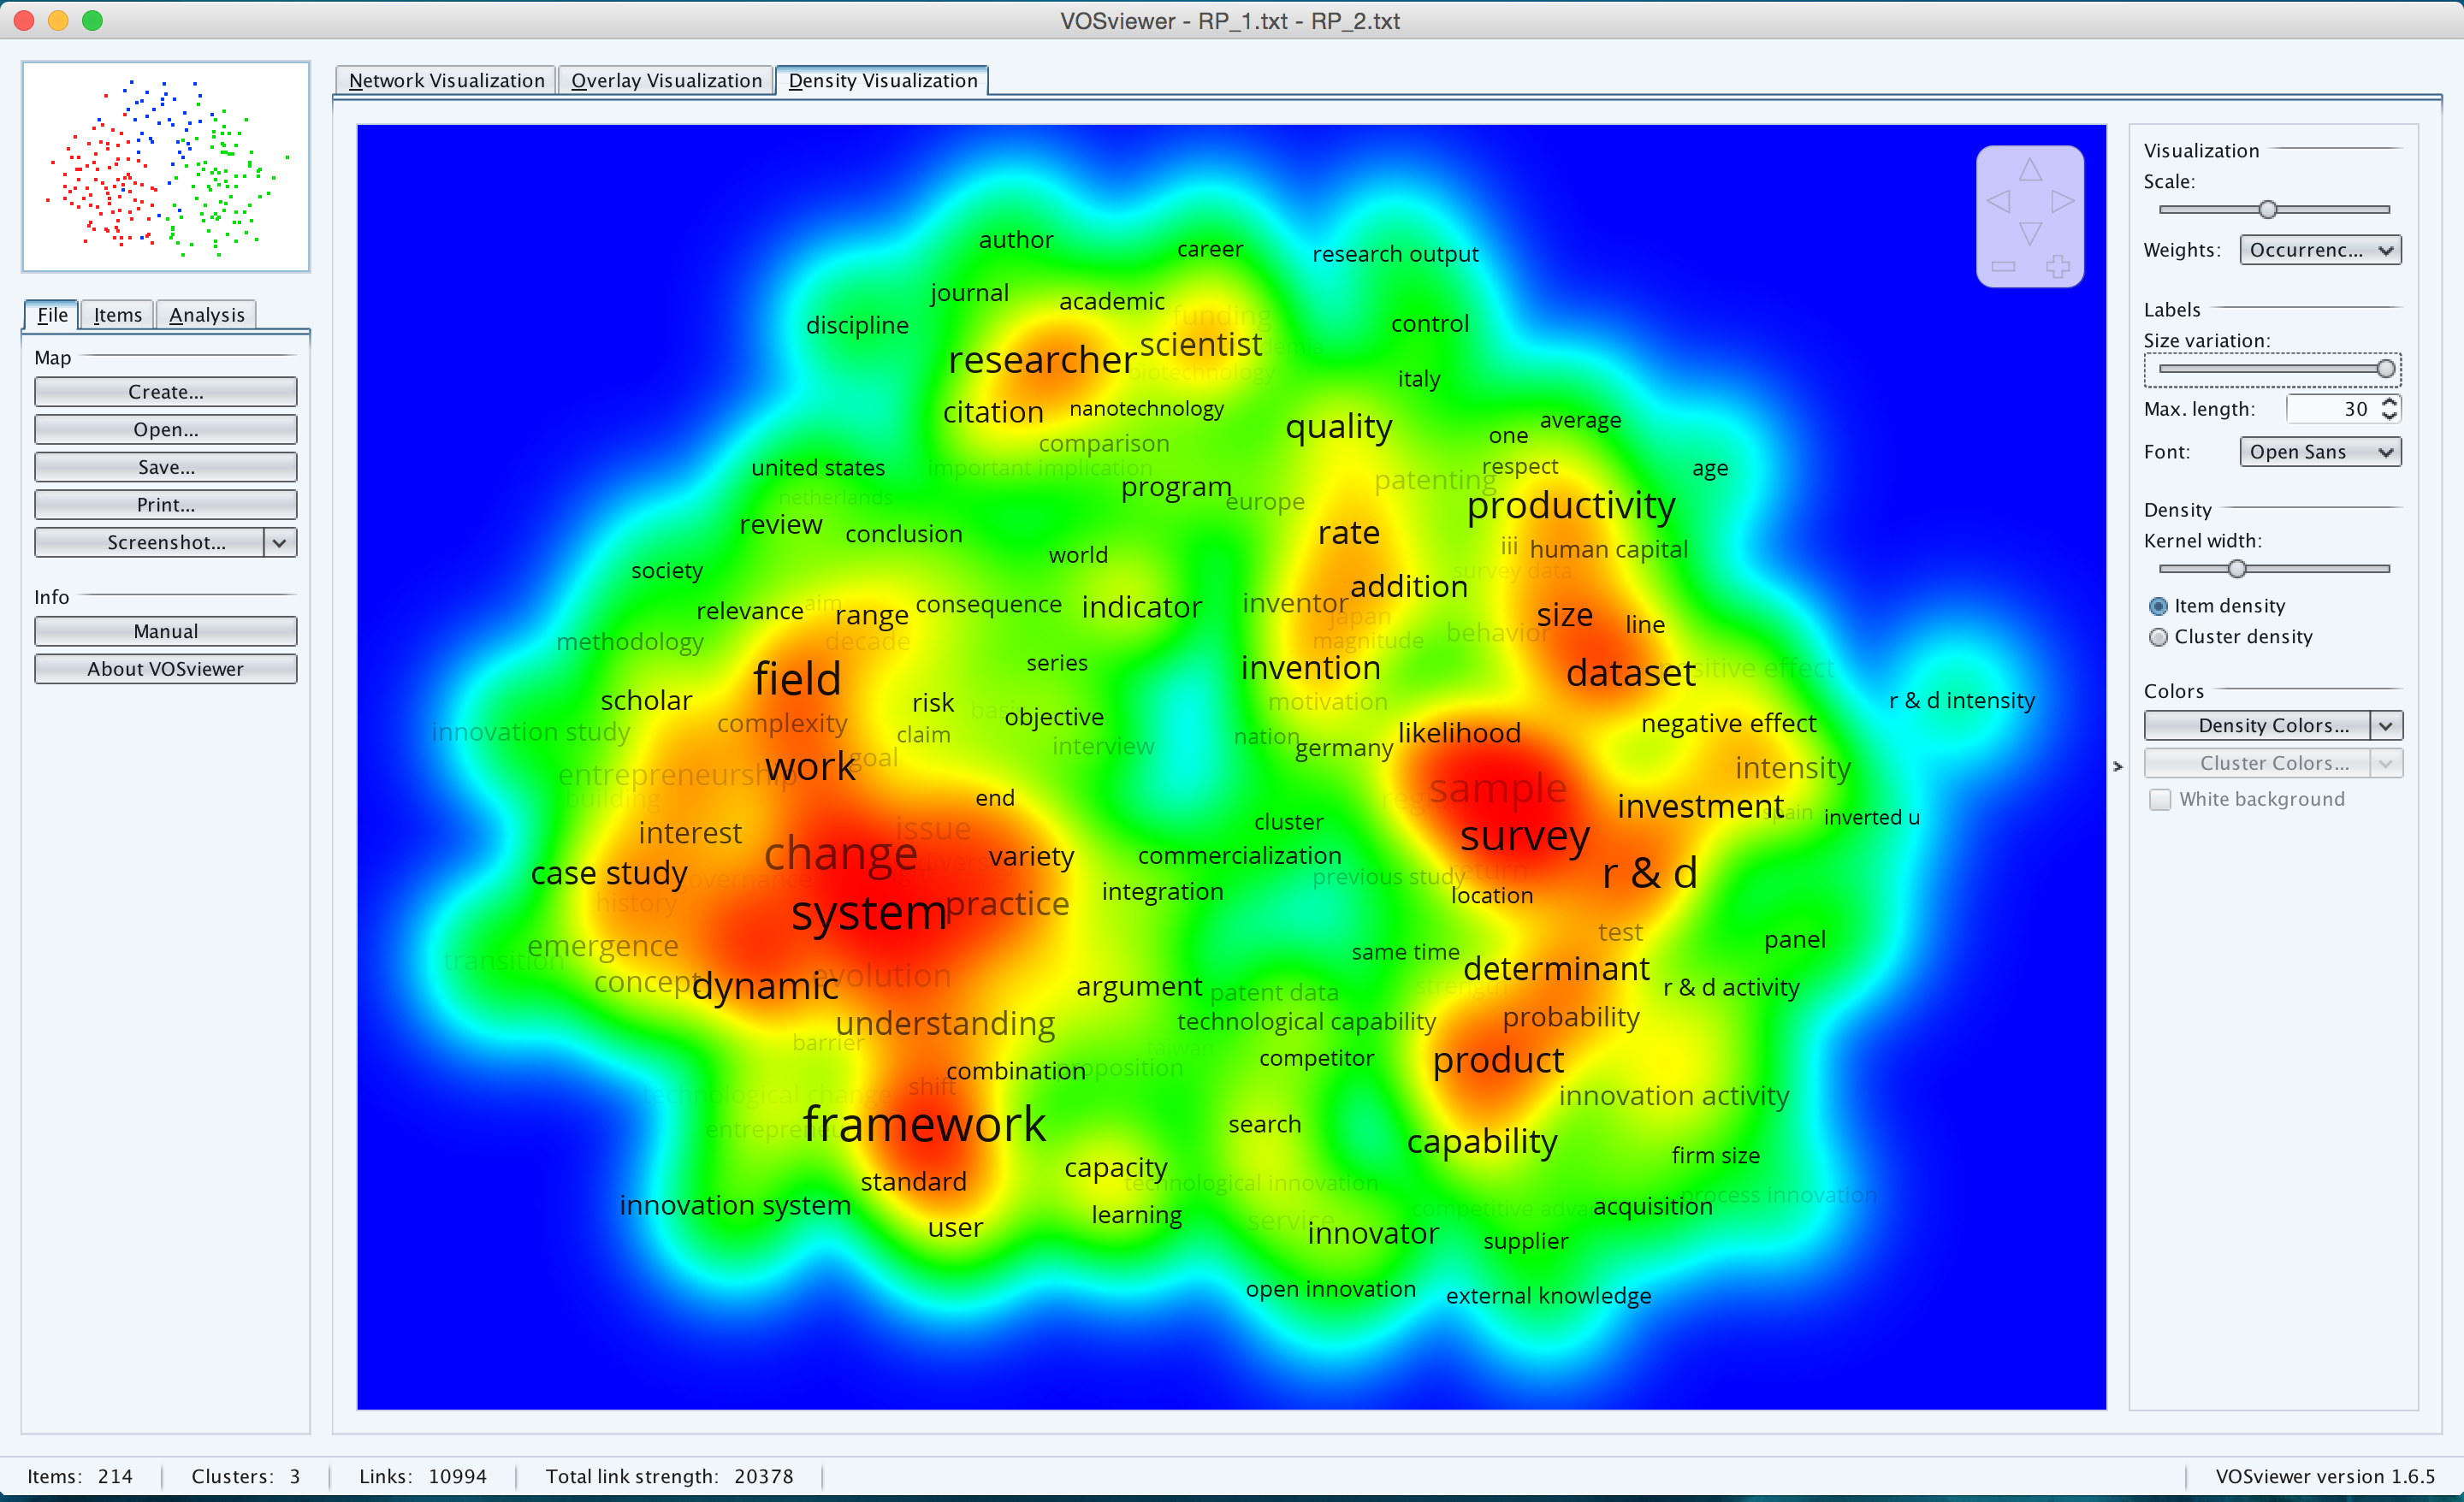
\includegraphics[width=\linewidth, frame]{vos}

\end{frame}

%------------------------------------------------

\begin{frame}
\frametitle{\insertsection}
\framesubtitle{Example}

\begin{columns}
\column{.5\textwidth}

\begin{itemize}
\item Let's examine the {\color{blue}{Research Policy's publications}} over the years 2008-2018
\item We can search these publications in {\color{blue}{Web of Science}} with the following search string: \\
	\medskip
	{\small SO=``Research Policy'' AND PY=(2018 OR 2017 OR 2016 OR 2015 OR 2014 OR 2008)}
	\medskip
\item This search returns {\color{blue}{1545 publications}} 
\item We downloaded the {\color{blue}{full records}}
\item We can upload these files in {\color{blue}{VOSviewer}}
	\begin{itemize}
	\item Create
	\item Create a map using bibliographic data
	\item Select the type of map
	\end{itemize}

\end{itemize}


\column{.5\textwidth}
\centering
\only<1>{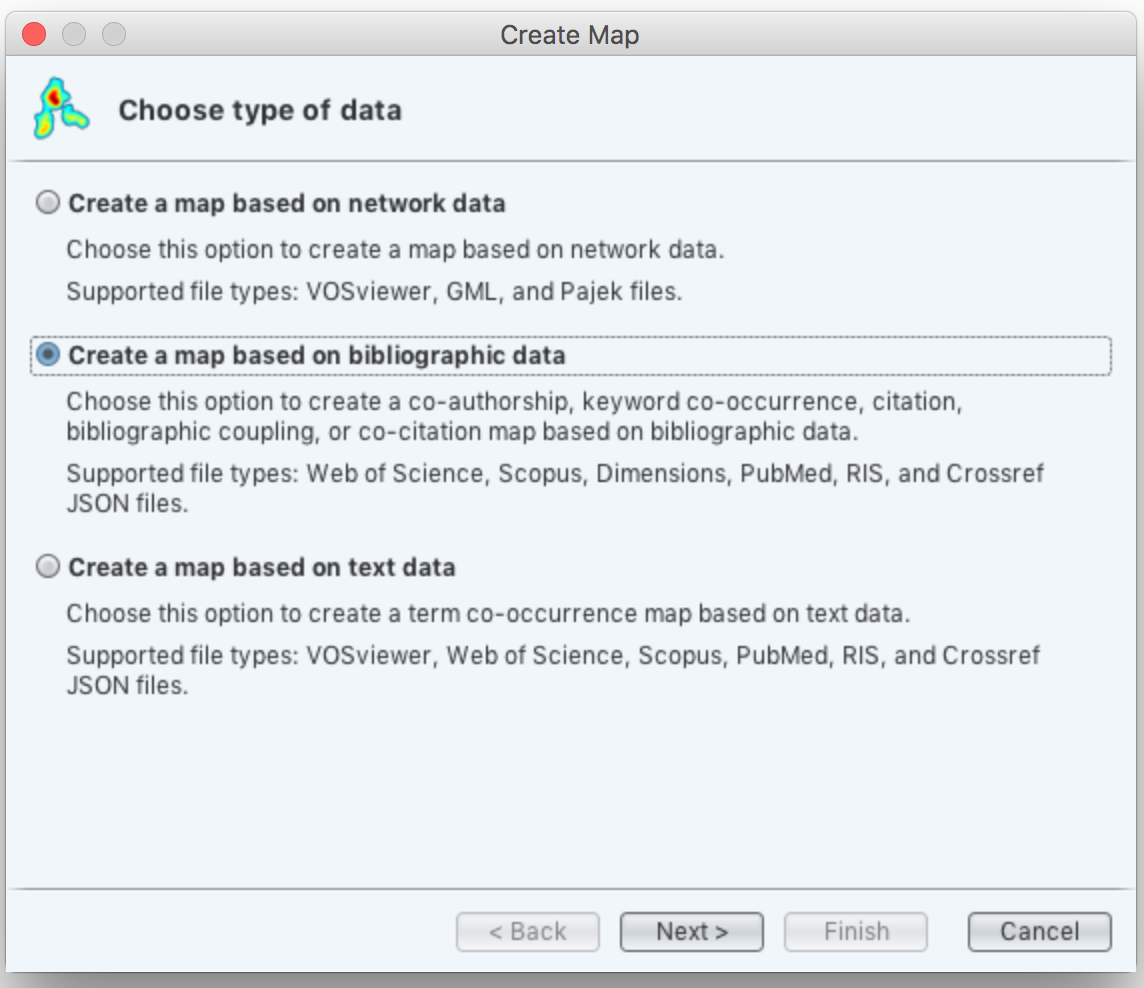
\includegraphics[width= \textwidth]{create1}}
\only<2>{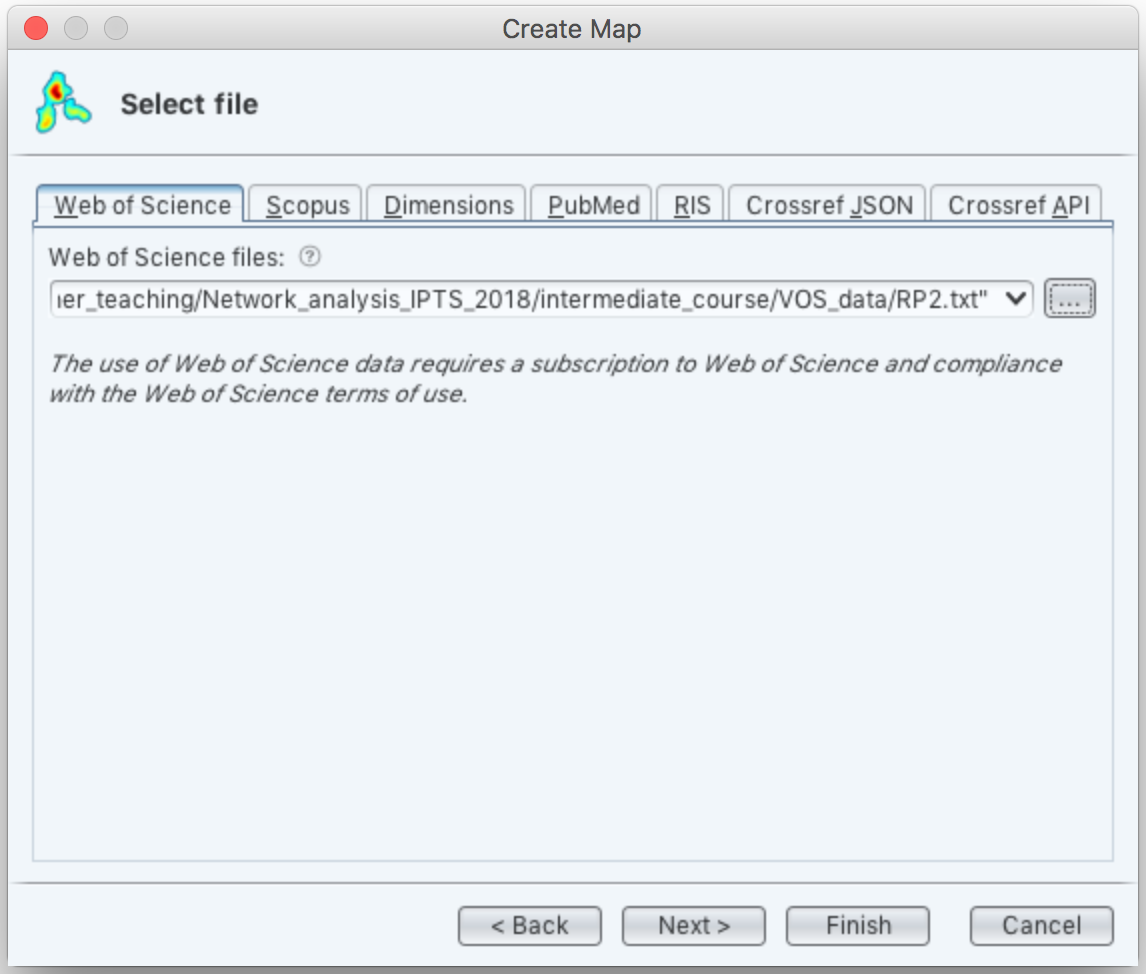
\includegraphics[width= \textwidth]{create2}}
\only<3>{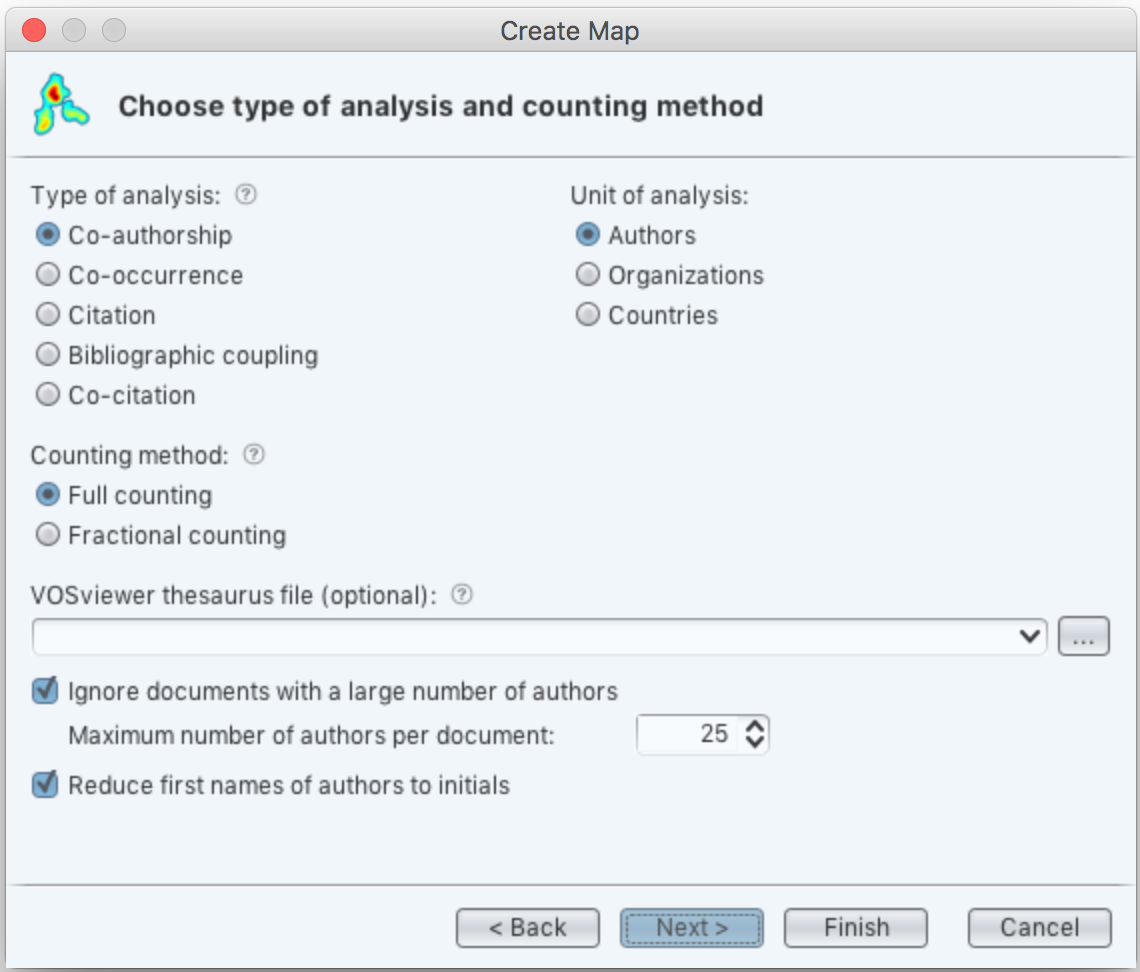
\includegraphics[width= \textwidth]{create3}}

\end{columns}

\end{frame}

%------------------------------------------------

\begin{frame}
\frametitle{\insertsection}
\framesubtitle{Example: Co-citation analysis}

\centering
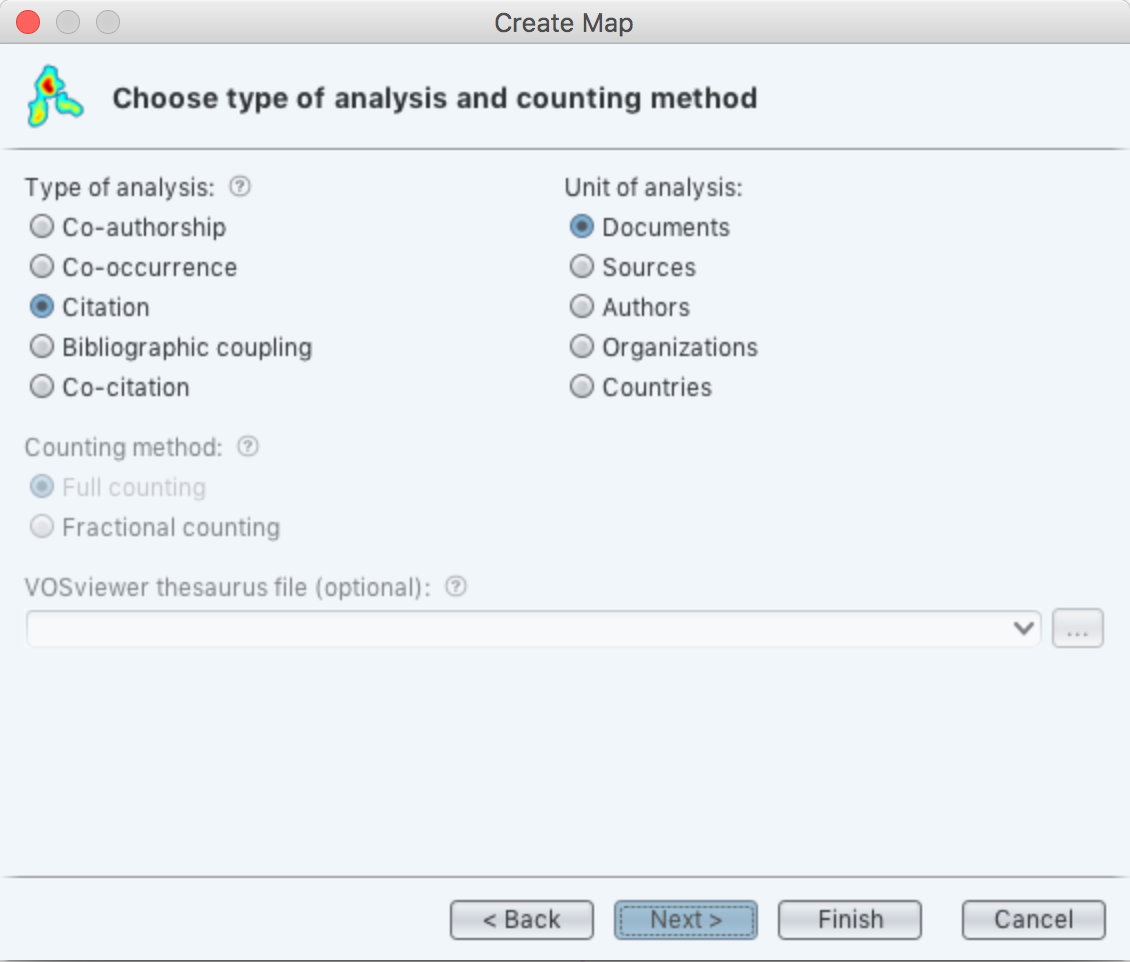
\includegraphics[width= 0.5\textwidth]{voscocitation}

\end{frame}

%------------------------------------------------

\begin{frame}
\frametitle{\insertsection}
\framesubtitle{Example: Co-citation analysis}

\centering
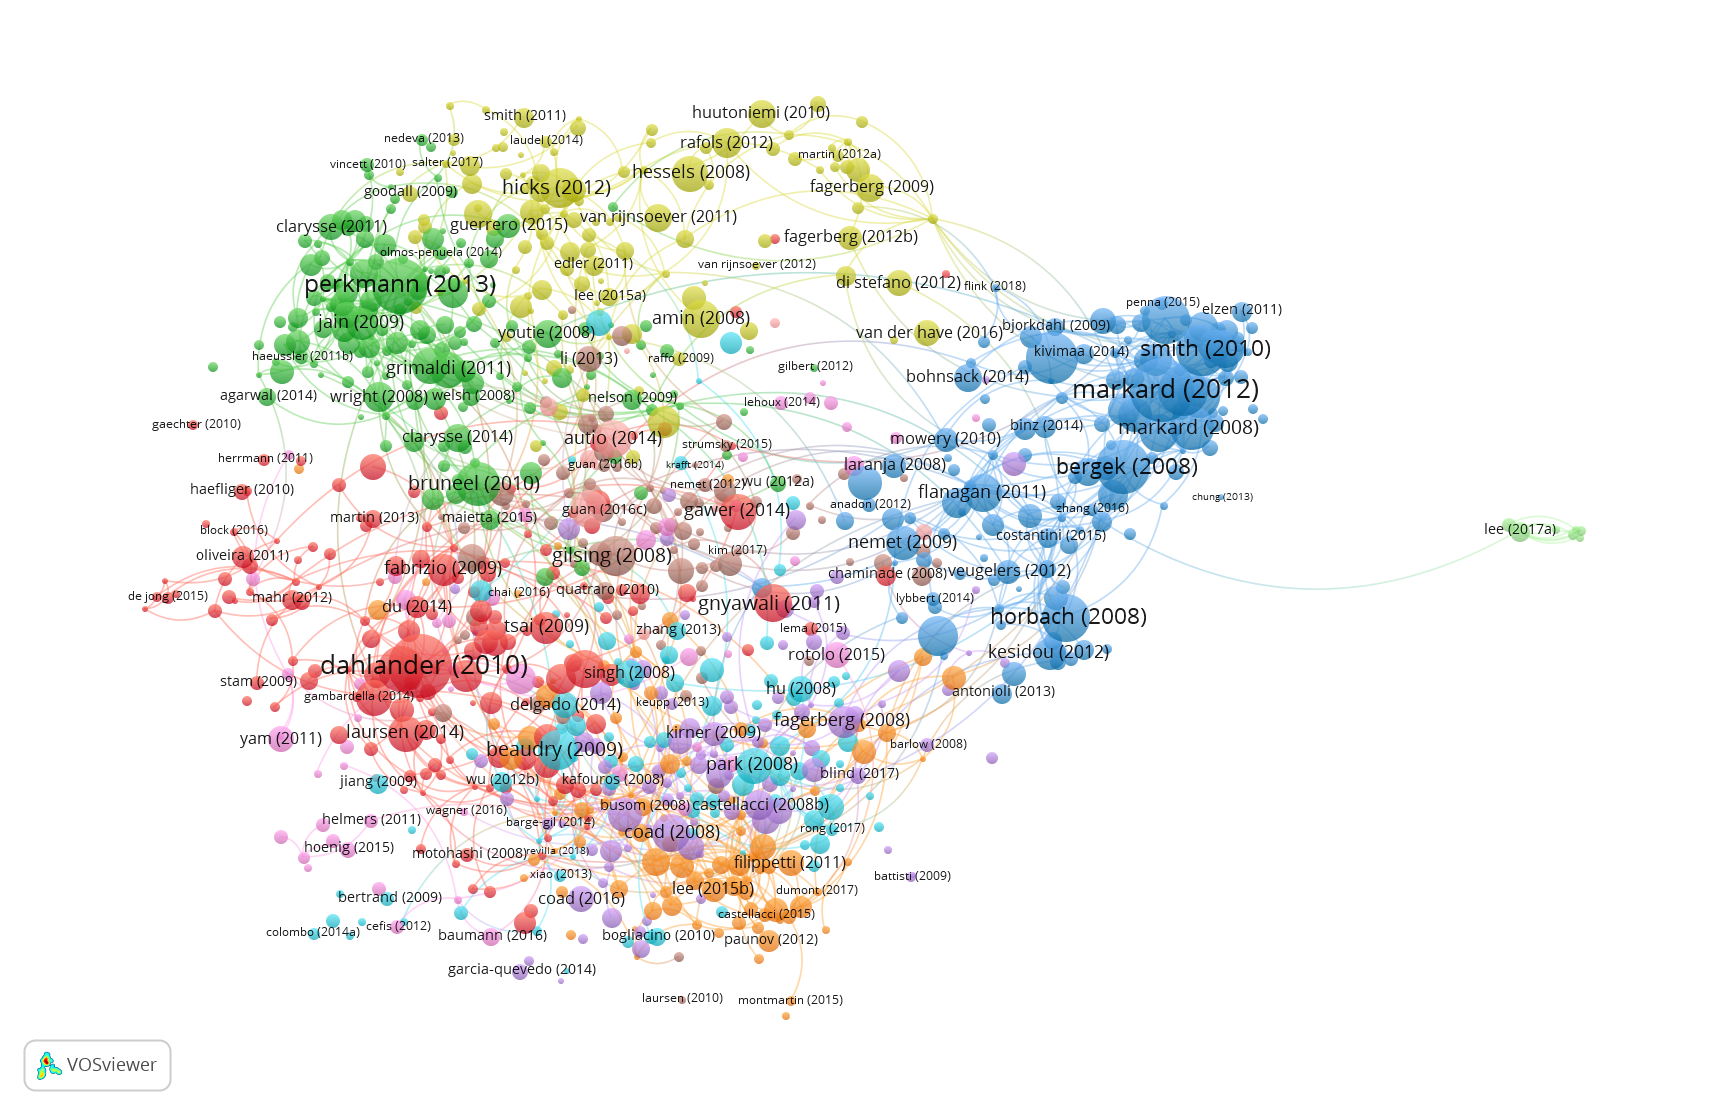
\includegraphics[height = 0.8\textheight]{RP_20082018_cocitation}

\end{frame}

%------------------------------------------------


\begin{frame}
\frametitle{\insertsection}
\framesubtitle{Example: Bibliographic coupling}

\centering
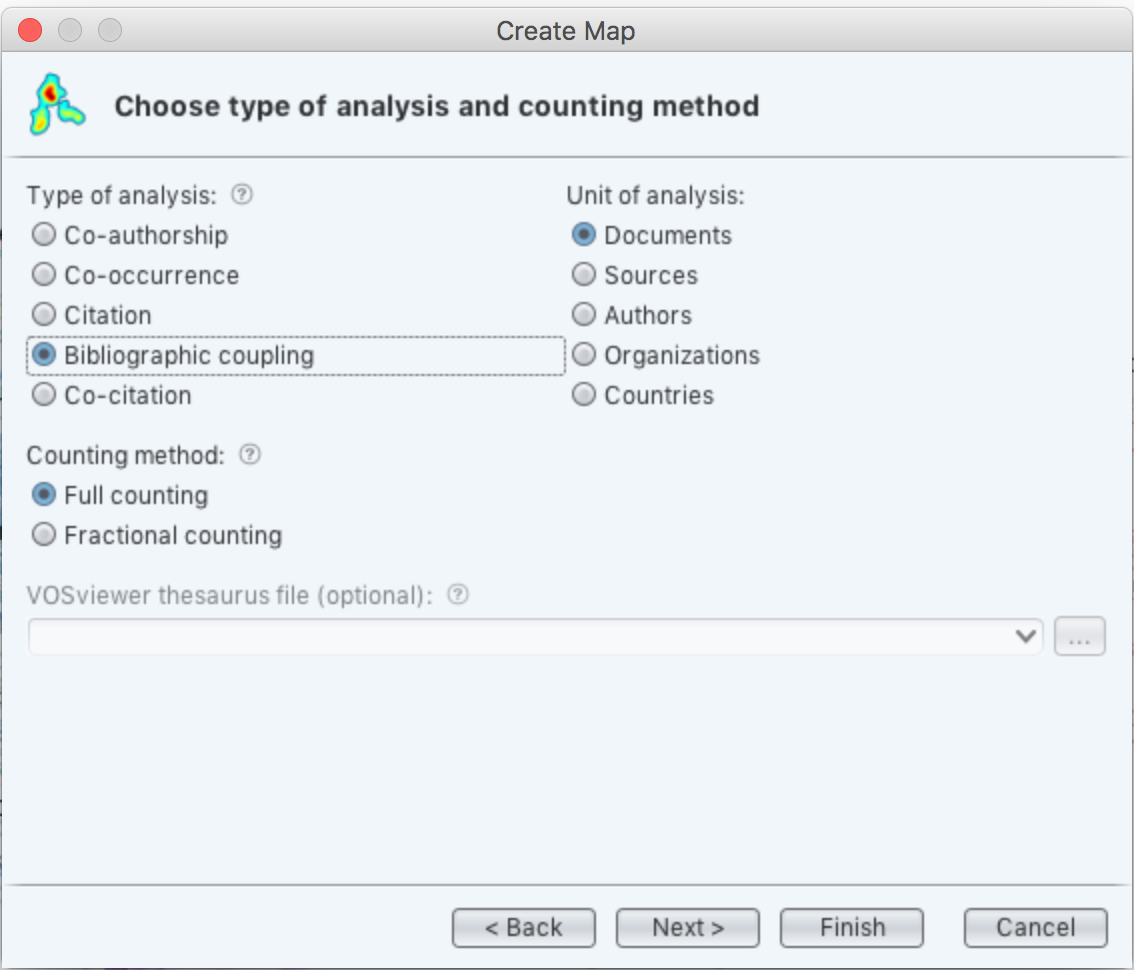
\includegraphics[width= 0.5\textwidth]{vosbiblio}

\end{frame}

%------------------------------------------------

\begin{frame}
\frametitle{\insertsection}
\framesubtitle{Example: Bibliographic coupling}

\centering
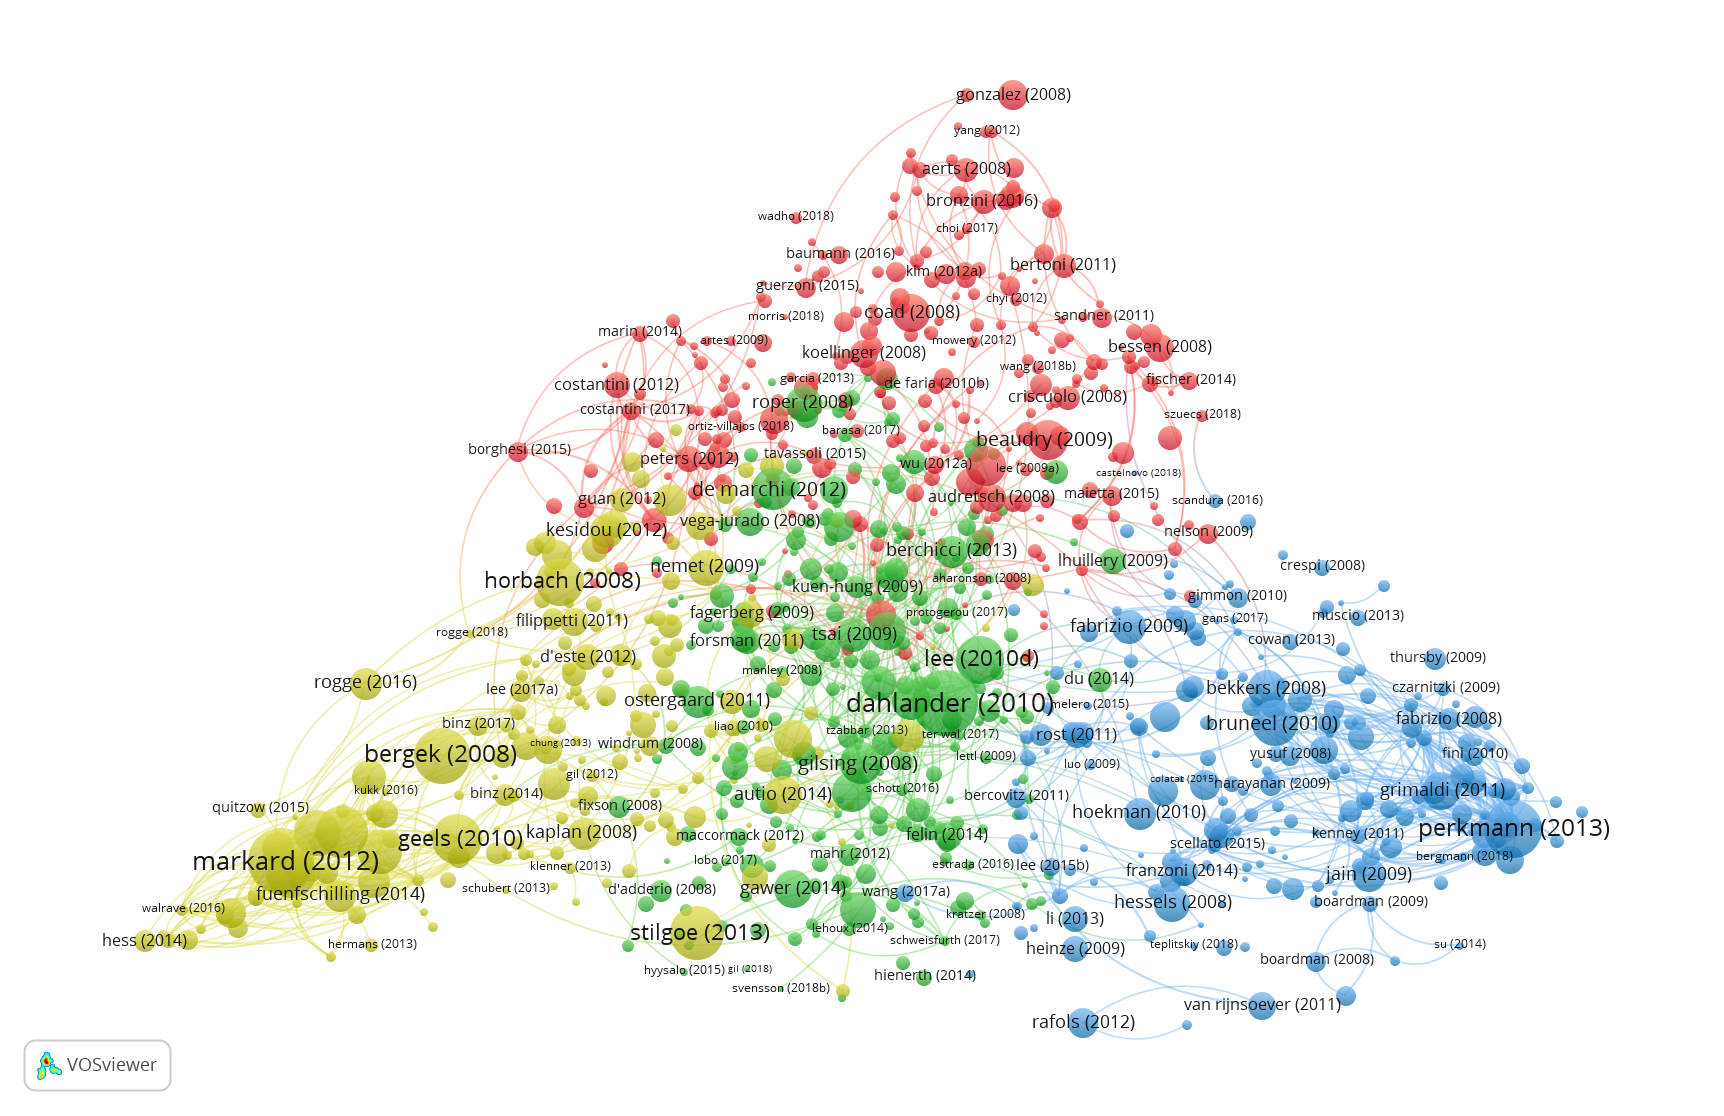
\includegraphics[height = 0.8\textheight]{RP_20082018_bibcoupling}

\end{frame}

%------------------------------------------------

\begin{frame}
\frametitle{\insertsection}
\framesubtitle{Example: How RP papers' references are jointly cited?}

\centering
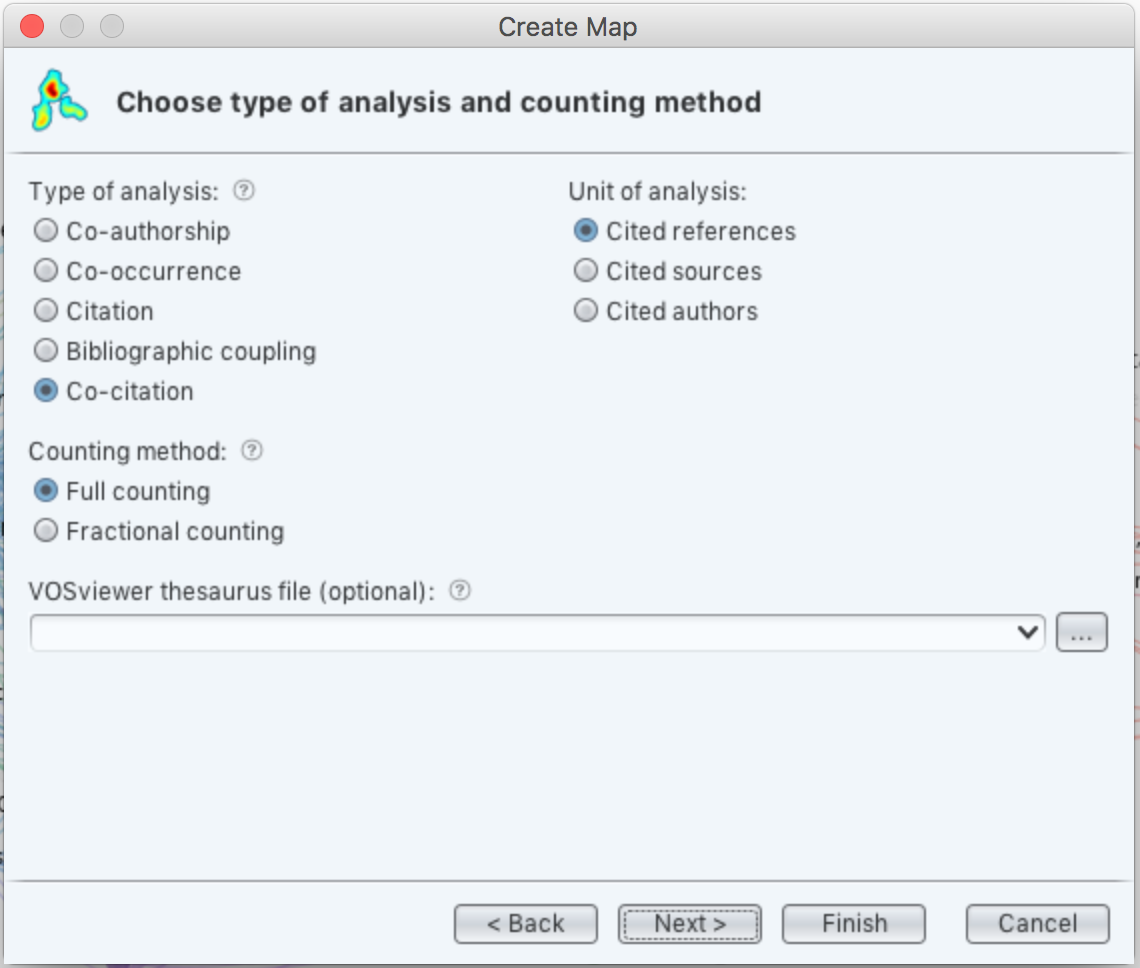
\includegraphics[width= 0.5\textwidth]{voscocitation_ref}

\end{frame}

%------------------------------------------------

\begin{frame}
\frametitle{\insertsection}
\framesubtitle{Example: How RP papers jointly cite their references?}

\centering
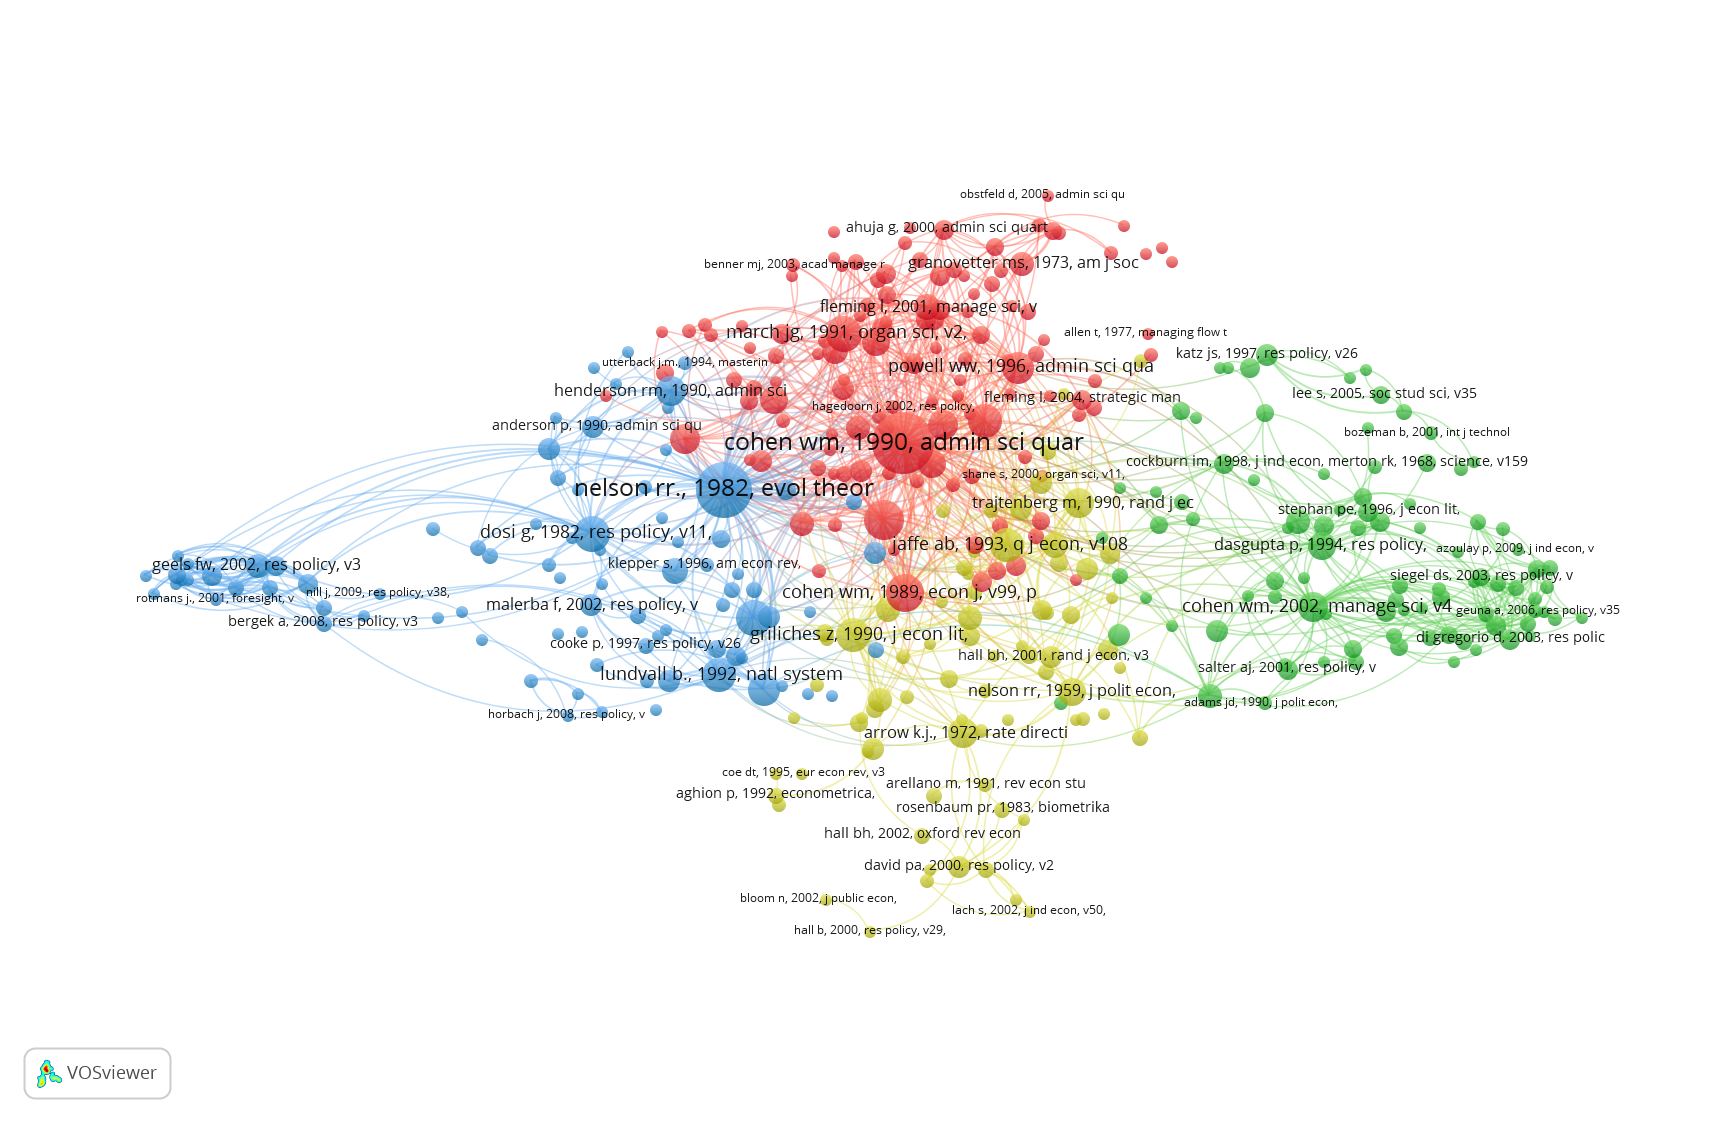
\includegraphics[height = 0.9\textheight]{RP_20082018_jointly_cited_references}

\end{frame}

%------------------------------------------------

\begin{frame}
\frametitle{\insertsection}
\framesubtitle{Example: Co-word analysis}

\centering
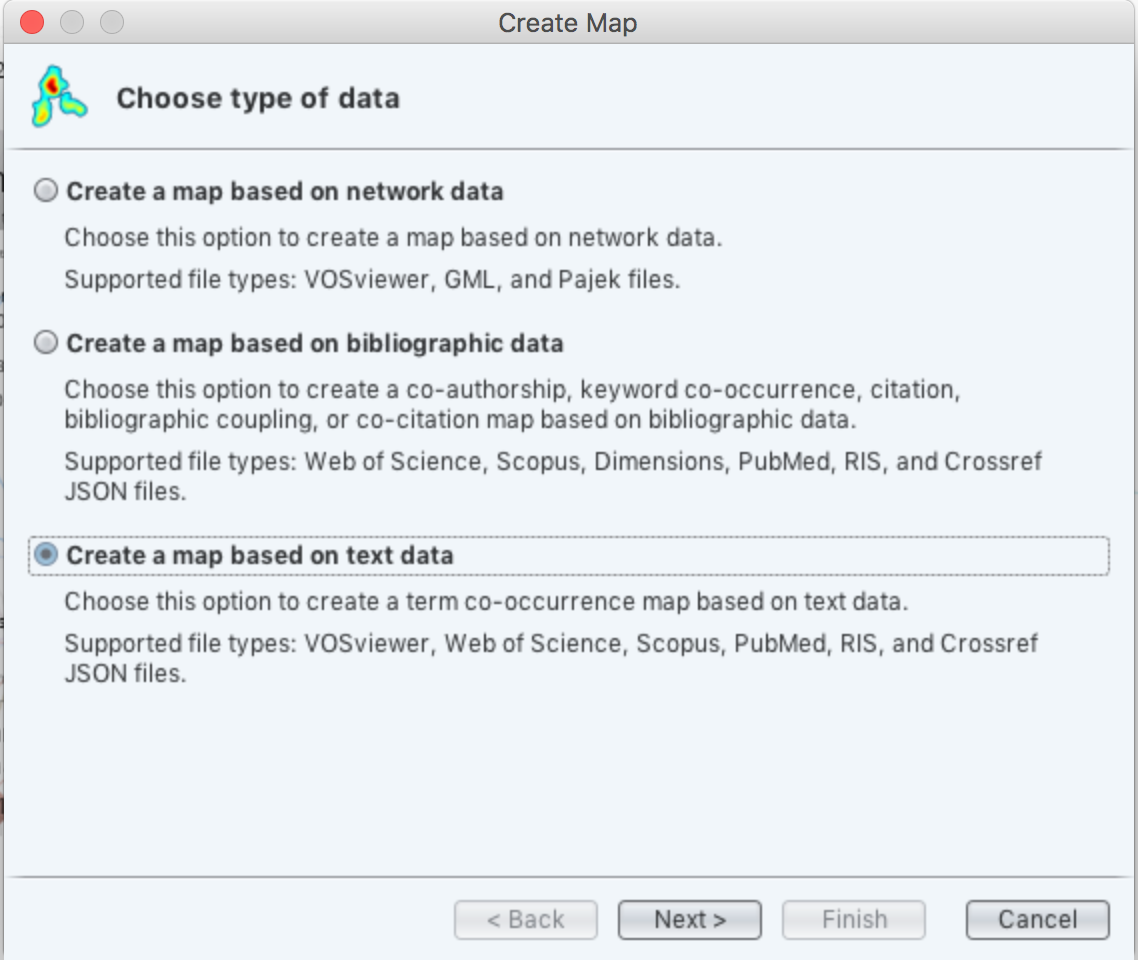
\includegraphics[width= 0.5\textwidth]{voscoword}

\end{frame}

%------------------------------------------------

\begin{frame}
\frametitle{\insertsection}
\framesubtitle{Example: Co-word analysis}

\centering
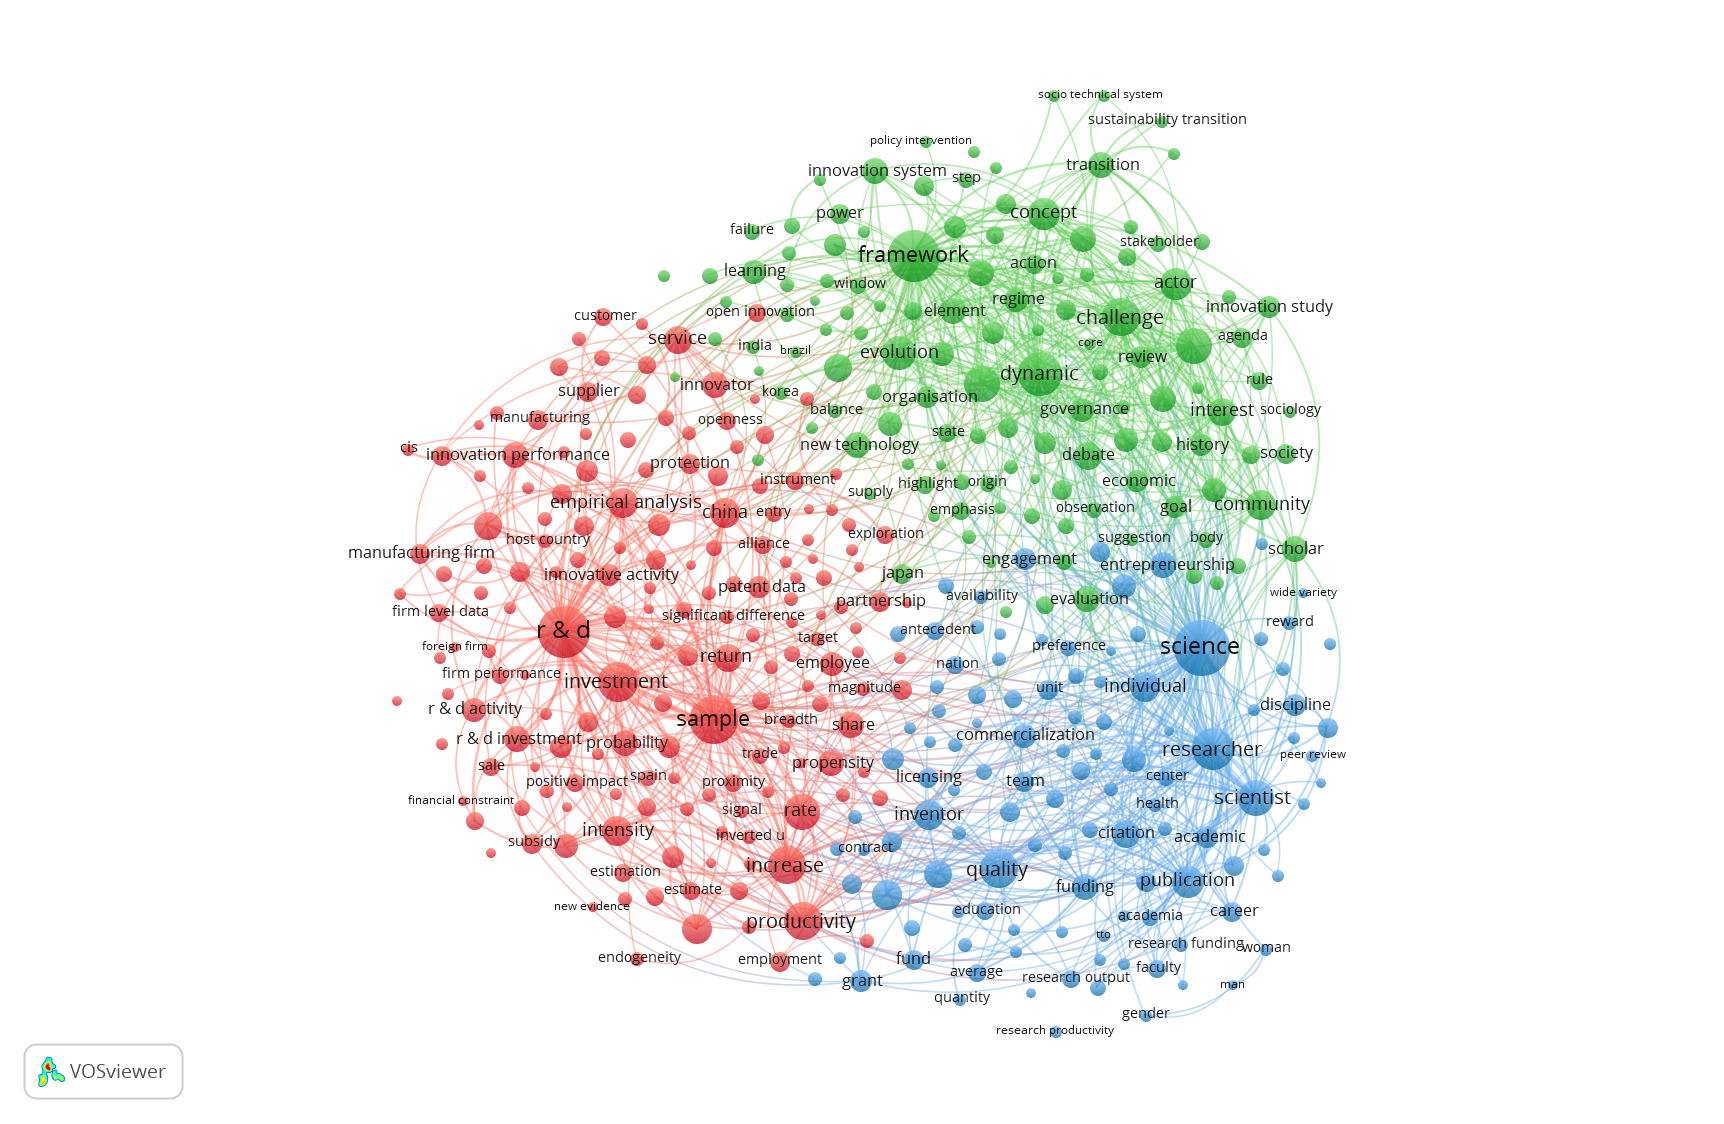
\includegraphics[height = 0.8\textheight]{RP_20082018_coword}

\end{frame}

%------------------------------------------------

\begin{frame}
\frametitle{\insertsection}
\framesubtitle{Exercise}

\textbf{Scientometric analysis in VOSviewer}
\medskip

\begin{enumerate}
\item Download a {\color{blue}sample of publications} that are of your interests from Web of Science
\medskip

\item For example, these can include
	\begin{itemize}
	\item publications of a specific journal
	\item publications related to a topic
	\item publications of a specific author
	\item publications of a country/region
	\item ...
	\end{itemize}
\medskip
	
\item Create and export the corresponding
	\begin{itemize}
	\item {\color{blue}co-citation} map
	\item {\color{blue}bibliographic coupling} map
	\item {\color{blue}co-word coupling} map
	\end{itemize} 

\end{enumerate}

\end{frame}

%------------------------------------------------

%------------------------------------------------

\begin{frame}
	\frametitle{\insertsection}
	\framesubtitle{Downloading bibliographic data from Web of Science}
	
	\textbf{How to download a sample of publications from Web of Science:}
	\medskip
	
	
	\begin{enumerate}
		\item Go to \url{https://apps.webofknowledge.com/}
		\item Search by keywords, authors, journals... 
		\item Once you have obtained the search results, refine your search by year, discipline...
		\item In the document type window, choose only "Articles"
		\item Export file using other formats: choose .txt (plain text format)  - You can export only 500 results per download!
		\item Export the full record and cited references 
		\item The data will look extremely messy if opened, but it's ready to be read in VOSviewer
	\end{enumerate}
	
\end{frame}

%------------------------------------------------








%%=======================================================
%	Questions
%%=======================================================
\section*{Questions}

%------------------------------------------------

\bgroup
\setbeamercolor{background canvas}{bg = navyblue}
\begin{frame}[plain]{}
\begin{center}
\color{white}{\Huge\insertsection}
\end{center}
\end{frame}
\egroup

%------------------------------------------------





%%=======================================================
%	Next time ...
%%=======================================================
\section*{Next time ...}
%------------------------------------------------

\bgroup
\setbeamercolor{background canvas}{bg = navyblue}
\begin{frame}[plain]{}
\begin{center}
\color{white}{\Huge\insertsection}
\end{center}
\end{frame}
\egroup

%------------------------------------------------

\begin{frame}
\frametitle{\insertsection}

\begin{itemize}

\item 	\textbf{Lecture: Social network theories}
	\begin{itemize}
	\item Social capital
	\item Strength of weak ties
	\item Structural holes
	\end{itemize}

		
\end{itemize}

\end{frame}

%------------------------------------------------







\end{document}